\chapter{Psalm 31}

\begin{figure}
  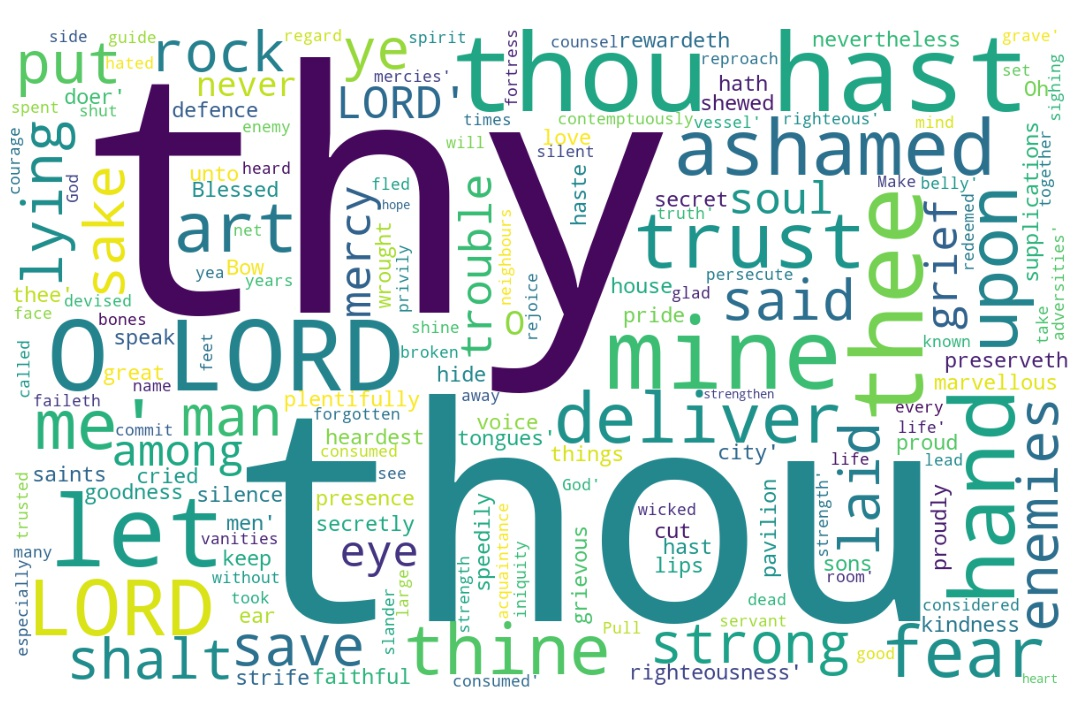
\includegraphics[width=\linewidth]{19OT-Psalms/Psalm31-WordCloud.jpg}
  \caption{Psalm 31 Word Cloud}
  \label{fig:Psalm 31 word Cloud}
\end{figure}


\marginpar{\scriptsize \centering \fcolorbox{bone}{lime}{\textbf{DAVID'S CRY}}\\ (Psalm 31:1--24) 
\begin{compactenum}[I.][8]
    \item \textbf{Special Trust} \index[scripture]{Psalms!Psa 031:01}(Psa 31:1)  
    \item \textbf{Secret Traps} \index[scripture]{Psalms!Psa 031:04}(Psa 31:4)  
    \item \textbf{Singular Trouble} \index[scripture]{Psalms!Psa 031:07}(Psa 31:7)  
    \item \textbf{Slandered Times} \index[scripture]{Psalms!Psa 031:13}(Psa 31:13)  
    \item \textbf{Sovereign Troops} \index[scripture]{Psalms!Psa 031:15}(Psa 31:15)  
    \item \textbf{Striving Tongues} \index[scripture]{Psalms!Psa 031:20}(Psa 31:20)  
    \item \textbf{Silenced Troublemaker} \index[scripture]{Psalms!Psa 031:23}(Psa 31:23)  
\end{compactenum} }

\footnote{\textcolor[cmyk]{0.99998,1,0,0}{\hyperlink{TOC}{Return to end of Table of Contents.}}}\footnote{\href{https://audiobible.com/bible}{\textcolor[cmyk]{0.99998,1,0,0}{Psalms Audio}}}\textcolor[cmyk]{0.99998,1,0,0}{To the chief Musician, A Psalm of David.}\\
\\
\textcolor[cmyk]{0.99998,1,0,0}{In thee, O LORD, do I put my \fcolorbox{bone}{lime}{trust}; let me never be ashamed: deliver me in thy righteousness.}
[2] \textcolor[cmyk]{0.99998,1,0,0}{Bow down thine ear to me; deliver me speedily: be thou my strong rock, for an house of defence to save me.}
[3] \textcolor[cmyk]{0.99998,1,0,0}{For thou \emph{art} my rock and my fortress; therefore for thy name's sake lead me, and guide me.}
[4] \textcolor[cmyk]{0.99998,1,0,0}{Pull me out of \fcolorbox{bone}{lime}{the net} that they have laid privily for me: for thou \emph{art} my strength.}\footnote{\textbf{Psalm 9:15} - The heathen are sunk down in the pit that they made: in the net which they hid is their own foot taken.}\footnote{\textbf{Psalm 25:15} - Mine eyes are ever toward the LORD; for he shall pluck my feet out of the net.}\footnote{\textbf{Psalm 66:11} - Thou broughtest us into the net; thou laidst affliction upon our loins.}\footnote{\textbf{Proverb 1:17} - Surely in vain the net is spread in the sight of any bird.}\footnote{\textbf{Proverb 12:12} - The wicked desireth the net of evil men: but the root of the righteous yieldeth fruit.}
[5] \textcolor[cmyk]{0.99998,1,0,0}{Into thine hand I commit my spirit: thou hast redeemed me, O LORD God of truth.}
[6] \textcolor[cmyk]{0.99998,1,0,0}{I have hated them that regard lying vanities: but I trust in the LORD.}
[7] \textcolor[cmyk]{0.99998,1,0,0}{I will be glad and rejoice in thy mercy: for thou hast considered my \fcolorbox{bone}{lime}{trouble}; thou hast known my soul in adversities;}
[8] \textcolor[cmyk]{0.99998,1,0,0}{And hast not shut me up into the hand of the enemy: thou hast set my feet in a large room.}
[9] \textcolor[cmyk]{0.99998,1,0,0}{Have mercy upon me, O LORD, for I am in trouble: mine eye is consumed with grief, \emph{yea}, my soul and my belly.}
[10] \textcolor[cmyk]{0.99998,1,0,0}{For my life is spent with grief, and my years with sighing: my strength faileth because of mine iniquity, and my bones are consumed.}
[11] \textcolor[cmyk]{0.99998,1,0,0}{I was a reproach among all mine enemies, but especially among my neighbours, and a fear to mine acquaintance: they that did see me without fled from me.}
[12] \textcolor[cmyk]{0.99998,1,0,0}{I am forgotten as a dead man out of mind: I am like a broken vessel.}
[13] \textcolor[cmyk]{0.99998,1,0,0}{For I have heard the \fcolorbox{bone}{lime}{slander} of many: fear \emph{was} on every side: while they took counsel together against me, they devised to take away my life.}
[14] \textcolor[cmyk]{0.99998,1,0,0}{But I trusted in thee, O LORD: I said, Thou \emph{art} my God.}
[15] \textcolor[cmyk]{0.99998,1,0,0}{My times \emph{are} in thy hand: deliver me from the hand of mine \fcolorbox{bone}{lime}{enemies}, and from them that persecute me.}
[16] \textcolor[cmyk]{0.99998,1,0,0}{Make thy face to shine upon thy servant: save me for thy mercies' sake.}
[17] \textcolor[cmyk]{0.99998,1,0,0}{Let me not be ashamed, O LORD; for I have called upon thee: let the wicked be ashamed, \emph{and} let them be silent in the grave.}
[18] \textcolor[cmyk]{0.99998,1,0,0}{Let the lying lips be put to silence; which speak grievous things proudly and contemptuously against the righteous.}
[19] \textcolor[cmyk]{0.99998,1,0,0}{\emph{Oh} how great \emph{is} thy goodness, which thou hast laid up for them that fear thee; \emph{which} thou hast wrought for them that trust in thee before the sons of men!}
[20] \textcolor[cmyk]{0.99998,1,0,0}{Thou shalt hide them in the secret of thy presence from the pride of man: thou shalt keep them secretly in a pavilion from the strife of \fcolorbox{bone}{lime}{tongues}.}
[21] \textcolor[cmyk]{0.99998,1,0,0}{Blessed \emph{be} the LORD: for he hath shewed me his marvellous kindness in a strong city.}
[22] \textcolor[cmyk]{0.99998,1,0,0}{For I said in my haste, I am cut off from before thine eyes: nevertheless thou heardest the voice of my supplications when I cried unto thee.}
[23] \textcolor[cmyk]{0.99998,1,0,0}{O love the LORD, all ye his saints: \emph{for} the LORD preserveth the faithful, and plentifully rewardeth the \fcolorbox{bone}{lime}{proud doer}.}
[24] \textcolor[cmyk]{0.99998,1,0,0}{Be of good courage, and he shall strengthen your heart, all ye that hope in the LORD.}